\section{Nebenfächer}
\label{sec:nebenfach}
Für den physikalischen Part eures Studiums wär`s das jetzt erst mal. Euer Stundenplan sieht jetzt schon relativ voll aus, ist aber noch nicht ganz fertig. Zu euren physikalischen Fächern kommen nämlich noch die Nebenfächer hinzu.\\
Als Nebenfach ist prinzipiell jedes nicht--physikalische Fach zugelassen. Ihr könnt auch zwei Nebenfächer studieren, wobei ihr beachten müsst, dass ihr am Ende eures Studiums mindestens 16--22 Credit~Points nachweisen müsst. Eigentlich sind hier der Phantasie der Wahl keine Grenzen gesetzt, die folgenden Fächer haben sich jedoch als \enquote{Standards} etabliert\ldots{}\\
Für eine Menge Nebenfächer sind Studienpläne vorgesehen, an die ihr euch halten müsst. Diese könnt ihr im Prüfungsamt einsehen. Wenn ihr jedoch viel lieber ein anderes Nebenfach belegen wollt, wie etwa \enquote{Zoologie der ost-usbekischen Steppe}, dann scheut euch nicht, bei Professor Maruhn nachzufragen, ob es möglich ist, dieses zu belegen.\\
Ein kleiner Tipp zum Nebenfach ist, dass ihr es möglichst früh belegen solltet, damit ihr immer noch Zeit habt, es zu wechseln. Oder stellt euch vor, dass ihr Stochastik als Nebenfach gewählt habt und dann nach einem Monat bemerkt, dass die Wahrscheinlichkeit, dass ihr dieses Nebenfach bis zum Ende bringen werdet, gegen Null geht\ldots{} Außerdem beginnen die meisten Nebenfächer nur im Wintersemester, einige auch nur im Sommersemester. Informiert euch also rechtzeitig.
\von{Fritz}
\begin{figure}
	\centering
	
\includegraphics[width=0.4\textwidth]{\imgdir/bartender.jpg}
\end{figure}
\newpage
\subsection{Geophysik}
\label{subsec:geophysik}
Als Newton der Apfel auf den Kopf gefallen ist, kam ihm die Idee mit der Schwerkraft. Aber ist die wirklich überall gleich?Und als die Mauern von Troja zusammenstürzten, war das wirklich Poseidon? Und wieso dreht sich die Kompassnadel immer nach Norden? Oder tut sie das gar nicht?\\
All diese Fragen bekommst Du in der Physik, wenn überhaupt, nur am Rande erklärt, weil diese Sachen in den Bereich der \fach{Geophysik} gehören. Die Geophysik beschreibt unseren Planeten mit physikalischen Methoden. Dazu ist die Geophysik in verschiedene Unterbereiche eingeteilt, die sich nur mit einzelnen Teilen beschäftigen, dazu gehören die Bereiche Seismologie, Magnetismus, Schwerebeschleunigung und viele andere.\\
Aber warum soll ich jetzt Geophysik als Nebenfach machen? Und was kann ich damit anfangen? Naja, wenn Dich zum einen unser Planet interessiert, dann bietet es sich an, ein bisschen mehr darüber zu erfahren. Und wenn Du später in der freien Wirtschaft arbeiten willst, hast du mit Geophysik gute Chancen. Mit der Angewandten Geophysik kannst Du zum Beispiel Bodenschätze suchen und finden oder den Untergrund für Hochhäuser erforschen.\\
\begin{figure}[!h]
 	\centering
  	
\includegraphics[width=.6\textwidth]{\imgdir/newton.jpg}
\end{figure}
Im ersten Modul Geophysik A (\Modul{GPA}), das Voraussetzung für die anderen beiden ist, erhälst Du mit der Vorlesung \VL{Einführung in die Geophysik} vorab einen Überblick über die Themen. Zu dieser Vorlesung gehört eine Übung, die Ihr besuchen müsst. Dazu kommen noch zwei weitere Vorlesungen, in denen Du Dich in einzelnen Bereichen spezialisierst. Eine der beiden Vorlesungen muss eine Übung haben. Abgeschlossen und benotet wird das Modul mit einer schriftlichen oder mündlichen Prüfung. Für dieses Modul erhälst Du 10 CP.\\
Das zweite Modul Geophysik B (\Modul{GPB}) setzt sich aus drei weiterführenden Vorlesungen zusammen, welche Du Dir ebenso wie die weiteren Vorlesungen im Modul \Modul{GPA} aussuchen kannst. Dadurch erhälst Du einen tieferen Einblick in die einzelnen Bereiche. Zu einer dieser Vorlesungen müsst Ihr an einer Übung teilnehmen. Ein Seminar, in dem Ihr selbst ein Thema auswertet und präsentiert, vervollständigt das Modul. Meistens wird das übergeordnete Thema vorgegeben und Du kannst dann aus einer Reihe von Themen wählen. Dabei betreut Dich einer der Professoren. Abgeschlossen und benotet wird das Modul wieder durch eine mündliche oder schriftliche Prüfung und Du erhälst auch hierfür 10 CP.\\
Als drittes Modul Geophysik C (\Modul{GPC}) gibt es ein Praktikumsmodul, bei dem Du richtige Messungen machst. Dabei kannst Du zwischen einem Laborpraktikum oder einem Feldpraktikum wählen. Bei dem Laborpraktikum machst Du verschiedene Versuche während des Semesters. Zu einem Versuch musst Du ein ausführliches Protokoll schreiben. Dieses Protokoll wird dann kontrolliert und ist der Abschluss dieses Moduls. Entscheidest Du Dich für das Feldpraktikum, fährst über vier Tage ins Gelände, machst Messungen und wertest diese anschlie\ss end aus. Die vier Versuche werden unter Anleitung eines Professors in Gruppen von ca 10 Studierenden gemacht. Zu einem ausführlichen Protokoll, das Abschluss des Moduls ist, musst Du eine weitere Vorlesung aus dem Bereich der Angewandten Geophysik hören. Das Feldpraktikum ist zwar somit mehr Aufwand, lohnt sich aber auf jeden Fall. Für dieses Modul erhälst Du nach dem erfolgreichen Protokoll unbenotet 5 CP.\\
Geophysik ist also die Physik richtig Anwenden und macht eine Menge Spa\ss . Solltest Du Dich für Geophysik als Nebenfach entscheiden, hast Du sicher keine falsche Wahl getroffen.
\von{bur}
\subsection{Astrophysik}
\label{subsec:astro}
Es ist ein warmer Sommerabend und du bist mit deinen Freunden am Strand oder in einem Park unterwegs und ihr schaut euch die Sterne an. Während alle anderen nur das romantische Bild des Himmels genie\ss en, überlegst du dir, wie weit der Stern ganz im Süden wohl ist, ob es überhaut ein Stern oder doch ein Plantet ist, was in seinem Inneren vorgeht? Wenn dir diese Situation bekannt vorkommt, ist \fach{Astronomie} als Nebenfach das Richtige für dich. Hier lernt man, das Universum physikalisch zu verstehen. Das bedeutet, es ist kein Nebenfach für reine Sterngucker, die möglichst viele hübsche bunte Bilder sehen wollen (keine Angst, die gibt es aber natürlich auch), sondern man beschäftigt sich mit Strahlungsprozessen, den Geschehnissen in unserer Sonne und unserem Planetensystem. Gerade das Kapitel Strahlung wirkt zu Beginn leicht abschreckend, stellt aber nach anfänglichen Schwierigkeiten kein grö\ss eres Problem dar.\\
Mit \fach{Astronomie} als Nebenfach könnt ihr bis zu 25 CP's sammeln und damit sogar die 22 CP, die ihr maximal für den Bachelor braucht, abdecken. Dabei ist es in zwei Module aufgeteilt: Das erste Modul, welches euch 12 CP gibt, besteht aus zwei Vorlesungen, die ihr ohne Probleme in den ersten beiden Semestern hören könnt. Dort werdet ihr euch vor allem mit der Sternentwicklung, Planetensystemen, unserer Sonne und Galaxien beschäftigen. Im zweiten Modul müsst ihr eine Spezialvorlesung hören und an einem Praktikum sowie einem Seminar teilnehmen. Im Allgemeinen kann man das Praktikum, welches nur im Sommersemester angeboten wird, schon im 2. Semester machen, da die einzige Voraussetzung die \VL{Astro1} Vorlesung ist. Somit könnt ihr mit eurem Nebenfach nach dem 3. Semester fertig sein, was insofern ganz praktisch ist, da man in den höheren Semestern noch Wahlpflichtveranstaltungen belegen muss, wofür man so mehr Zeit hat. Au\ss erdem ist der Praktikumsinhalt auf die 2. Vorlesung abgestimmt, ihr könnt damit also sehr leicht euer Wissen verfestigen. Zum Ende des 2. Semesters kommen nun endlich auch die Sternegucker unter euch auf ihre Kosten. Im Rahmen des Praktikums wird eine Beobachtungsnacht auf dem kleinen Feldberg veranstaltet, bei der ihr viele der von euch zuvor theoretisch untersuchten Objekte auch mal live sehen könnt. Für das Modul \Modul{AstroB} erhaltet ihr 13CP's.
%Gehalten werden alle Vorlesungen und das Praktikum von Professor T. Boller, der eigentlich am MPE, dem Max-Planck-Institut für extraterrestrische Physik in Garching bei München, arbeitet und jeweils einmal pro Woche an die Universität Frankfurt kommt.
%Dies weist den Vorteil auf, dass er an aktuellster Forschung beteiligt ist, was in der Vorlesung seinen Einfluss findet.
\von{Patricia}
\begin{figure}[!t]
 	\centering
  	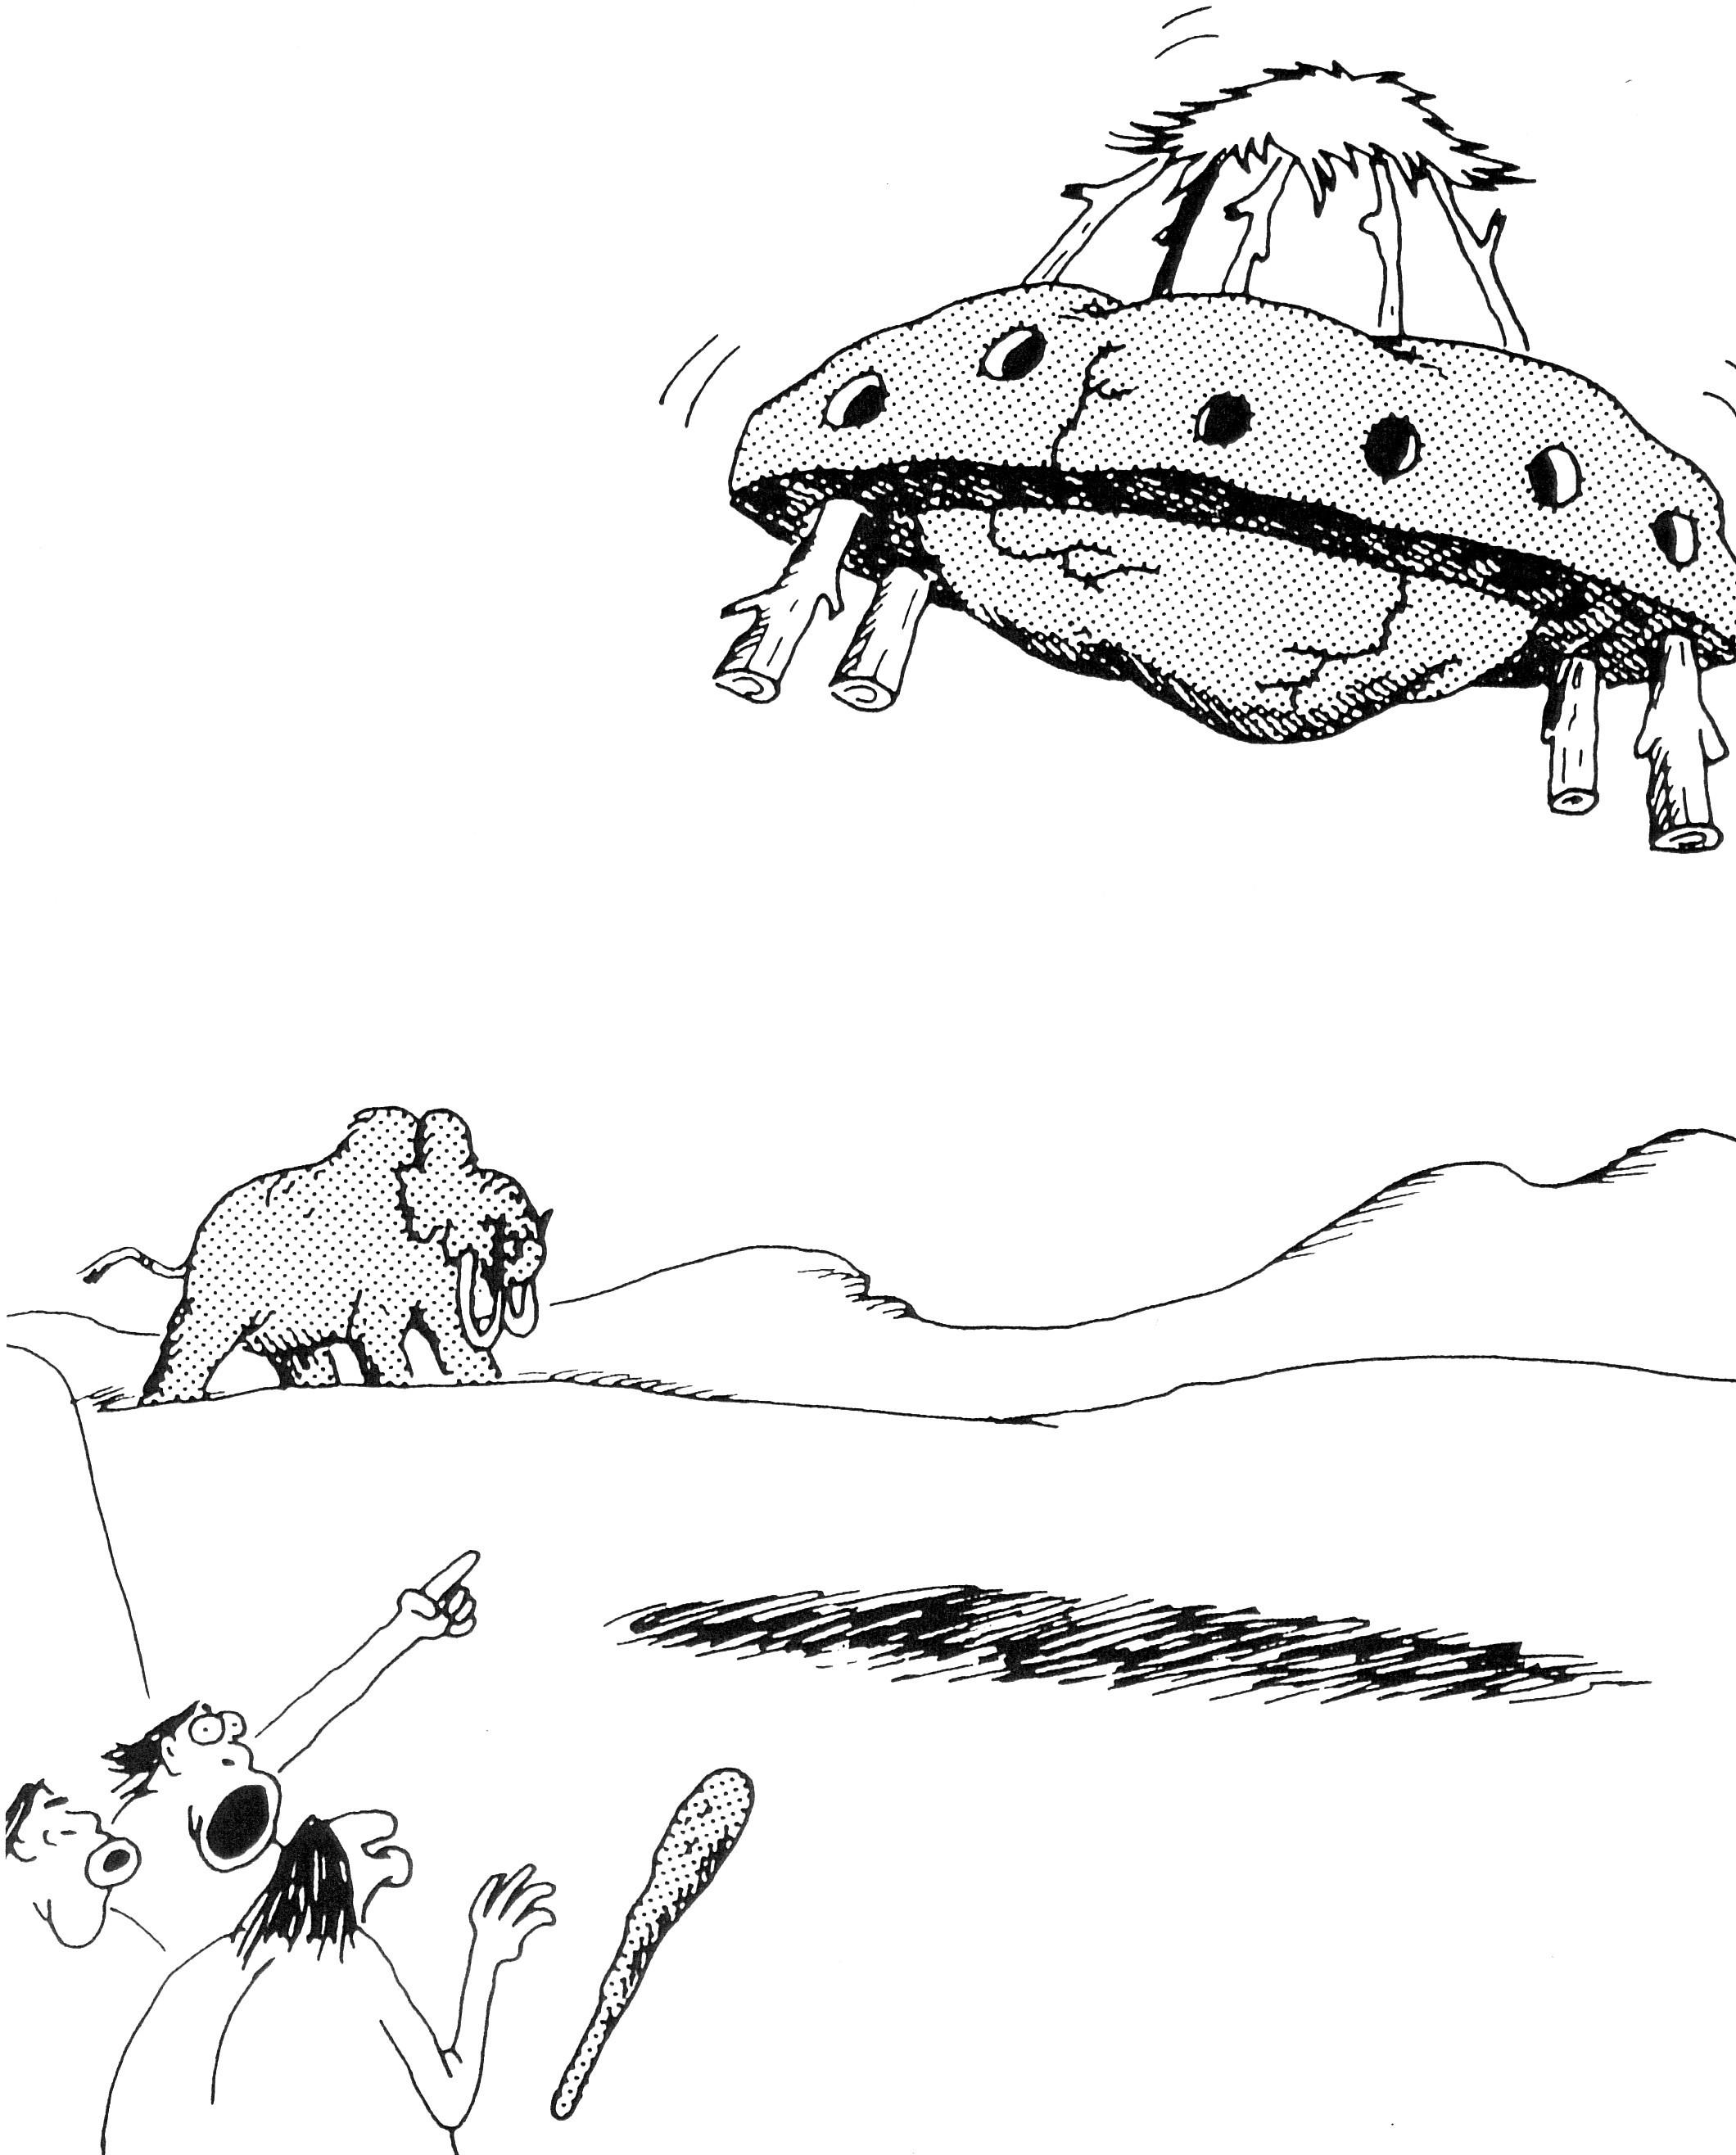
\includegraphics[width=.4\textwidth]{\imgdir/steinufo.jpg}
\end{figure}
\subsection{Meteorologie}

Ich persönlich studiere Meteorologie auf Diplom und Physik auf Bachelor, habe daher selber Meteorologie als Nebenfach belegt. 
Im Folgenden möchte ich euch dieses Fach als Nebenfach vorstellen.\\
\fach{Meteorologie} ist ein sehr interessantes Fach, da es ziemlich viel mit Physik zu tun hat, das Thema aber einmal von einer anderen Perspektive angeht.
Es handelt sich dabei um eine noch sehr wenig erforschte Wissenschaft, die man aber im alltäglichen Leben leichter beobachten kann als einige andere Nebenfächer, die an der
Uni Frankfurt angeboten werden.\\
Nun aber zu den Inhalten und den Dingen, die ihr für dieses Fach leisten müsst.\\
Laut Bachelor - Prüfungsordnung können alle Module der bestehenden Bachelorordnung des Bachelorstudiengangs Meteorologie gewählt werden.\\
Ihr fangt mit dem Modul \Modul{EMet A} an.
Dieses umfasst die Vorlesungen \VL{Allgemeine Meteorologie} und \VL{Klimatologie} und gibt insgesamt 10 CP.\\
In der allgemeinen Meteorologie geht es z.B. um meteorologische Grundbegriffe, die Struktur der Atmosphäre und um Windgesetze. 
\begin{figure}[!t]
  \begin{center}
  
\includegraphics[width=.7\textwidth]{bilder/meteorologe.jpg}
\end{center}
\end{figure}

\pagebreak

Die Klimatologie betrachtet nicht kurzlebige Phänomene wie das Wetter, sondern lange Zeiträume von mindestens 30 Jahren.
Prof. Dr. Bodo Ahrens erklärt, wie man Klima "`macht"', also wie man es mit statistischen Methoden bestimmt und welche meteorologischen Größen dabei eine Rolle spielen.
\bigskip

Danach könnt ihr mit dem Modul \Modul{EMet B} weitermachen.
Dafür bekommt ihr auch 10 CP.
\\Das Modul umfasst eine Einführung in die Theoretische Meteorologie (\VL{Atmospheric Dynamics I} und \VL{II}).
\\Die Theoretische Meteorologie beschäftigt sich unter anderem mit der Kinematik des Windfeldes, der Newtonschen Mechanik und mit Thermodynamik.
\bigskip

Mit dem Modul \Modul{EMet A} könnt ihr direkt im Wintersemester anfangen.
Es sind keine Vorkenntnisse notwendig.
\von{Luisa}

\subsection{Informatik}
%Im Unterschied zur Physik, die beschreibt "`was ist``, versucht die Informatik, Handlungsanweisungen und Konzepte zu geben, um grosse Datenmengen (Informationen) effizient verarbeiten zu können. Dazu werden in der Vorlesung grundlegende Konzepte für Handlungsanweisungen (Algorithmen), ihre sprachliche Formulierung (Programme) und ihre Informationen (Daten) vorgestellt und gelernt. Dies dient dazu, Struktur und Design sowie den Einsatzbereich verschiedener Programmiersprachen zu erkennen und einschätzen zu können, um für ein gegebenes Problem die geeignete programmtechnische Formulierung zu wählen. Aber auch den Lebenszyklus von Software und elementare Prozesse und Methoden der Software--Entwicklung lernen wir kennen. Weiterhin wird die Ablaufumgebung, also die typischen Konzepte und Eigenschaften von Betriebssystemen, erläutert, um bei Problemen konstruktiv eingreifen zu können. Dazu zählen beispielsweise die Problemfelder IT--Sicherheit und Netzwerke. Im zweiten Teil der Vorlesung werden die Programmiersprachenkonzepte von Syntax und Semantik um die Bereiche der funktionalen und objektorientierten Sprachen erweitert und damit das Verständnis von Programmiersprachen vertieft. Dazu kommt die Modellierung, Verwaltung und Nutzung großer Datenbestände mit Hilfe von Datenbanken.
%\von{Rüdiger Brause}


\fach{Informatik} ist ein durchaus nützliches Nebenfach, da das Programmieren oft ein wichtiges Hilfsmittel
für Physiker darstelllt. 
So vielseitig wie der Studiengang Informatik kann auch dieses Nebenfach werden, 
denn es lassen sich alle Module wählen und beliebig kombinieren. 
Will man das Fach einbringen, muss man jedoch die Vorlesung \VL{Grundlagen der Programmierung 1} (\Modul{PRG-1})
mit Übung belegen und die Klausur, die meist noch in der Vorlesungszeit geschrieben wird, bestehen.
Diese Vorlesung gibt einem einen guten und strukturierten Überblick über die Themengebiete der Informatik, 
sie ist aber gleichzeitig auch ein Schnupperkurs zur Programmierung.
Belohnt wird dies mit 11 CP.
Anschließend kann man, zum Beispiel im Sommersemester,
mit \VL{Datenstrukturen} oder \VL{Hardwarearchitekturen und Rechensysteme} weitermachen.
Das Nebenfach ist ab dem ersten Semester geeignet.
Da \Modul{PRG-1} nur im Wintersemester angeboten wird, ist es auch sinnvoll, damit gleich anzufangen.
\fach{Informatik} ist auf jeden Fall ein interessantes Nebenfach, sowohl für diejenigen mit Vorkenntnissen,
um diese zu strukturieren und zu vertiefen, als auch für diejenigen ohne Vorkenntnisse,
um einen Überblick über das Fachgebiet zu erhalten.
\von{Rita}

\begin{center}

  
\includegraphics[width=0.35\textwidth]{bilder/einstein.jpg}

\end{center}

\subsection{Geschichte der Naturwissenschaften}

Geschichte der Naturwissenschaften - was soll das den sein?
... Habe ich mir auch gedacht und bin einfach mal in der ersten Woche hingegangen.\\
Dieses Nebenfach besteht aus mehreren kleinen Seminaren mit jeweils zwei Stunden die Woche, ist also ziemlich gut neben den Pflichtvorlesungen zu machen.\\

Nun aber zum Inhalt:
In \fach{Geschichte der Naturwissenschaften} geht man der naturwissenschaftlichten Begriffs- und Theorienbildung auf den Grund.
Woher kommen zum Beispiel die Begriffe \textit{Kraft} und \textit{Energie}?
Wie hat sich unser Weltbild im Laufe der Jahrtausende langsam entwickelt?
Worin sind unsere heutigen Denkstrukturen begründet?
Wenn ihr diese Fragen interessant findet, ist \fach{Geschichte der Naturwissenschaften} wirklich sehr zu empfehlen.\\

Im Moment unterteilt sich das Fach noch in zwei Module, von denen eines 12 CP und eines 13 CP liefert:\\
Das 12 CP - Modul trägt den Titel \Modul{Einführung in die Naturphilosophie}.
Wie der Name schon sagt, beschäftigt man sich hier in drei eher philosophischen Seminaren mit den Anfängen wissenschaftlichen Denkens.
Haupsächlich wird hier die Antike behandelt.\\
Das 13 CP - Modul heißt \Modul{Einführung in die Geschichte der Naturwissen- schaften}.
Auch dieses Modul teilt sich wieder in drei Seminare auf, deren Themen von Semester zu Semester variieren.
Relativ oft wird die klassische Mechanik im 17. und 18. Jahrhundert behandelt.
Ansonsten betrachtet man die Originaltexte einzelner Mathematiker und Physiker dieser Zeit.
Oft werden die Texte auch in der Original-Sprache vorgelegt, interessant, wenn man in der Schule Französich oder Latein gelernt hat.
Das ist allerdings keine Voraussetzung, es gibt auch immer Übersetzungen zumindest ins Englische.\\

Jedes Seminar ist benotet.
Wie die Note zustande kommt, hängt allerdings am Dozenten:
Es kann also ein Kurzvortrag sein oder auch eine Hausarbeit.\\

Das Nebenfach lässt sich in drei Semestern abschließen.
Alles in allem ist \fach{Geschichte der Naturwissenschaften} ein sehr angenehmes Nebenfach, das eine willkommene Abwechslung zum Pflichtbereich ist.

\von{Miriam}

\subsection{Elektronik}
\label{subsec:elektronik}
Das Nebenfach \fach{Elektronik} besteht aus zwei Modulen, die beide belegt werden müssen. Mit beiden kann man innerhalb von zwei Semestern 16 Credit Points bekommen.\\
Das Nebenfach fängt immer im Wintersemester an mit \Modul{Elek1}.
Darin enthalten sind zwei Vorlesungen. \VL{Elektronik und Sensorik} (2 SWS + 1 SWS Übung) im Wintersemester und im darauffolgenden Sommersemester die Vorlesung \VL{Digitalelektronik} (2 SWS). Parallel dazu läuft im Sommersemester ein Praktikum, das Modul \Modul{Elek2}. Das ist wiederum in einen Digital- und einen Analogteil aufgeteilt. Die Credit Points gibt es, wenn man alle Protokolle mit OK zurück hat und eine mündliche Prüfung zu den Vorlesungen hinter sich hat, wobei diese Note als Note für das komplette Nebenfach zählt. In Elektronik ist man meist in einer recht überschaubaren Gruppe, was eine gute Lernatmosphäre schafft.\\
Zu den Themen:\\
Die Analogelektronik beschäftigt sich erst mal mit den grundlegenden elektronischen Bauteilen, wie Widerstand, Spule, Kondensator und den hieraus bestehenden Schaltungen (sogenannte lineare passive Netzwerke). Danach kommen die Halbleiterbauelemente wie Dioden, Bipolartransistoren und Feldeffektransistoren etc dran, sowie eine Einführung in die Sensorik.\\
In der Digitalelektronik werden diese Bauteile dann genutzt um logische Schaltungen aufzubauen, welche mit Boolscher Algebra beschrieben werden können. Au\ss erdem werden Zustandsautomaten, Speicher und Mikroprozessoren besprochen. Hier erhält man sehr interessante Einblicke in das Innenleben von Computern.\\
Allerdings kommt man um einiges an Mathematik nicht drum herum. Deswegen hat man auf jeden Fall einen Vorteil, wenn man schon ein Semester hinter sich hat und zumindest die Grundlagen der Elektrodynamik und Fourier-Analyse kennt. Wen es aber wirklich interessiert, für den sind sicher auch mangelnde Vorkenntnisse kein Problem! Also, einfach mal ausprobieren.
\von{Berit und Martin}
\subsection{Philosophie}
\label{subsec:philosophie}
\textit{\enquote{Ich wei\ss , dass ich nichts wei\ss !}}\\
Das wissen eigentlich alle oder? Warum also noch Philosophie studieren?\ldots Warum eigentlich \"uberhaupt irgendetwas machen? Warum handeln Menschen oder erst einmal: Gibt es uns Menschen denn? und wenn ja, was gibt es noch?
\begin{figure}[!b]
  	\centering
	
\includegraphics[width=.275\textwidth]{\imgdir/Ich_weiss.jpg}
\end{figure}
Viele Fragen gibt es in der Philosophie, das ist wohl wahr\ldots Aber halb so wild, denn was ist schon \enquote{Wahrheit}?\\\\
W\"ahlst du \fach{Philosophie} als Nebenfach, wirst du dich mit all diesen Fragen besch\"aftigen m\"ussen. Du wirst \"uber die Metaphysik und die Erkenntnistheorie diskutieren und du wirst dir bez\"uglich so mach einer Meinung die Hand vor den Kopf schlagen oder erstaunt die Augen \"offnen.\\
Das Philosophiestudium ist eines der vielseitigsten und wenn du denken und diskutieren magst, auch eines der spa\ss igsten \"uberhaupt. Und als Erg\"anzung f\"ur die sonst so klinischen Physiker-Nerds ideal geeignet.\\
Das gilt \"ubrigens auch anders herum. Es ist erstaunlich, wie oft dir in der Philosophie die Physik begegnet. Mein Tutor zog die Quantenmechanik mindestens einmal pro Stunde als Beispiel heran =)\\
Das Philosophiestudium beginnst du mit einem der Basismodule (\Modul{BM}).
Im \Modul{BM1} hast du 2x2 SWS Vorlesung und ein 1x2 SWS Tutorium.
Die Vorlesung sieht folgenderma\ss en aus:\\
Jeder Student kauft sich eine Mappe mit philosophischen Texten (auch online verf\"ugbar), welche gelesen werden m\"ussen und nach und nach in den Vorlesungen besprochen werden. Im Tutorium sieht man sich den Text dann noch genauer an und merkt, wie wenig man ihn eigentlich verstanden hat :P\\
Abgeschlossen wird das Modul durch eine Klausur und bringt dir dann 12 CP.\\
Auch sehr interessant ist es als Physiker \Modul{Logik} zu h\"oren. Hier lernt man n\"amlich, wie man logisch richtige Argumente hervorbringt und was zum Beispiel logische Fehlschl\"usse sind.\\
Dazu kannst du eines der \Modul{AM} (Aufbaumodule) belegen, welche 8CP's bringen. Welche \Modul{AM's} angeboten werden, kannst du im aktuellen Vorlesungsverzeichnis nachlesen. Als Besonderheit ist zu beachten, dass du als Nebenf\"achler alle Aufbaumodule besuchen darfst, auch wenn sie als Vorraussetzung Vorlesungen haben, die du nicht geh\"ort hast.
\von{Marco}
\subsection{Chemie}

Das klassische Physiker-Nebenfach ist eindeutig \fach{Chemie}. Das ist nicht 
verwunderlich, da sich die Themen oft gut erg\"anzen. \fach{Chemie} geh\"ort 
außerdem zu den Nebenf\"achern mit den meisten Modulen, sodass man sich aus 
einer grossen Auswahl zusammenstellen kann, was einen am meisten interessiert.
Oder man kombiniert mit einem anderen Nebenfach. Auf jeden Fall muss man die
Vorlesung \VL{Allgeime und anorganische Chemie}
(Modul \Modul{ChemA}) sowie ein Praktikum (Modul \Modul{ChemB} oder \Modul{PCP}) besuchen. Alle 
weiteren Module sind danach optional.\\
Ein grosser Vorteil dieses Nebenfachs ist zweifellos auch, dass die 
Chemie-Geb\"aude \glqq nebenan\grqq ~sind, d.h. Campus-Pendeln entf\"allt.
\\
\\
1.Semester:\\
Vorlesung \VL{Allgeime und anorganische Chemie}
(Modul \Modul{ChemA}, 7CP). \\
In dieser Vorlesung geht es allgemein um die Grundlagen 
der Anorganischen und Physikalischen Chemie. Im Prinzip: Atome und Molek\"ule,
Thermodynamik, chemisches Gleichgewicht, S\"auren und Basen, Elektrochemie 
und nat\"urlich einmal quer durchs Periodensystem - eine Auffrischung der 
der kompletten Schulchemie und mehr.\\
Am Ende des Semesters wird eine Klausur geschrieben, nach deren Ausgang die 
Praktikumspl\"atze vergeben werden. Diese Klausur ist aber kein Hindernis -
in der Regel schneiden Physiker dabei ganz gut ab.\\
Die Vorlesung selber teilen sich zwei Professoren: Prof. Auner,
Prof. Martin Schmidt und Prof Buchsbaum. Gewechselt wird um Weihnachten herum. Der erste Teil 
ist eher etwas trocken, aber der zweite Abschnitt kompensiert das ganz gut.
Dann werden auch mal Experimente vorgef\"uhrt und Anschauungsmaterial
mitgebracht.\\
Wer also schon immermal Silizium-Wafer in der Hand haben wollte, oder die 
Kristalle der verschiedenen Elemente und Verbindungen sehen wollte, der ist 
hier gut aufgehoben. Einige interessante Themen sind: \\
Gewinnung von Aluminium und Silizium, warum Diamant nicht ewig h\"alt, 
Funktionsweise von Laserdruckern und Kopierern, Photographie, Halbleiter ...
um nur ein paar Dinge zu nennen.\\
\\
Nachteile will ich auch nicht verschweigen: Zumindest am Anfang ist der 
H\"orsaal ziemlich voll, da diese Vorlesung f\"ur andere Studieng\"ange 
Pflichtveranstaltung ist. Ausserdem liegt die Vorlesung f\"ur Langschl\"afer
und Weitgereiste ung\"unstig, n\"amlich gleich Montag und Mittwoch von 
8-10 Uhr.\\
Zu dieser Veranstaltung wird eine \"Ubung (Teilnahme freiwillig) angeboten.\\
\\
2.Semester:\\
Praktikum \VL{Chemie f\"ur Naturwissenschaftler} (\Modul{ChemB}, 3,5CP)\\
Das Praktikum ist vierst\"undig angesetzt, aber wenn man es gut organisiert, 
braucht man wesentlich weniger Zeit. Es geht dabei haupts\"achlich um
 anorganische Chemie und ihre Anwendungen, wie z.B. Titration, 
Nachweisreaktionen, pH-Wert-Bestimmung und Trennmethoden. Insgesamt sind es 
acht Versuchstage und jeweils ein Seminar dazu. Auch hier wird am Ende wieder 
eine Klausur geschrieben, deren Stoff aber wesentlich weniger umfangreich ist,
als im ersten Semester. Bei den Versuchstagen ist Kitteltragen durchaus 
sinnvoll, sonst hat man pl\"otzlich L\"ocher in der Kleidung, wo eigentlich 
keine sein sollten. Insgesamt macht es viel Spaß, die verschiedenen 
L\"osungen zusammenzumixen und man erlebt dabei immer wieder \"Uberraschungen.\\
Als Alternative kann das Praktikum \VL{Physikalische Chemie} besucht 
werden (\Modul{PCP}, 5,5CP).\\
\\
Hier noch eine kleine Auswahl weiterf\"uhrender Module:\\
\Modul{Physikalische Chemie I} (Therm, 6CP),\\
\Modul{Organische Chemie} (Org, 7CP),\\
\Modul{Festk\"orperchemie} (ChemF, 3CP).\\
\\
Chemie ist auf jeden Fall ein lohnendes und interessantes Nebenfach, wenn man 
ein bisschen panschen will und sich auch f\"ur andere Naturwissenschaften 
interessiert, denn Chemie verbindet im Prinzip Physik, Biologie und 
Geowissenschaften miteinander. Super. 
\von{Kristin}

\subsection{Nuklearmedizin}  %wie viele CP es n\"achstes mal geben wird muss erst noch gekl\"art werden
\label{subsec:nuklearmedizin}
\enquote{Oh mein Gott, wir brauchen Hilfe! Ist ein Arzt anwesend?}\\
Auf diese Frage wolltest du schon immer einmal mit \enquote{Ja!} oder \enquote{Aus dem Weg, ich bin Arzt!} antworten?\\
Hm, ich auch, aber da hilft dir dieses Nebenfach nicht wirklich weiter. Auch wenn der Name es suggestiert, \fach{Nuklearmedizin} macht dich nicht zum Mediziner. Du lernst zwar etwas \"uber die Grundlagen der menschlichen Anatomie (Leber, Schilddr\"use und Co), aber im Wesentlichen geht es um die physikalischen Eigenschaften von Radionukliden und ihre Anwendungsm\"oglichkeiten in der Medizin. Hierzu besch\"aftigst du dich z.B. mit folgenden Fragen:
\begin{itemize}
  \item{Warum strahlen manche Stoffe?}
  \item{Was ist Strahlung \"uberhaupt und welche Varianten gibt es?}
  \item{Welche Strahlung wirkt wie auf die Zellen und warum?}
  \item{Wie schaffe ich es, dass genau der Bereich verstrahlt wird, den ich bestrahlen will und sonst keiner?}
  \item{Wie nutze ich Strahlung zur Diagnostik? (Detektorphysik)}
  \item{Wie lese ich CT/MRT oder PET Bilder?}
\end{itemize}
Und vielen weiteren. Alles in allem stellt es eine gelungene Symbiose aus Medizin, Zellbiologie und Physik dar und hilft dir, \"uber den (sowieso schon gro\ss en, aber immer noch erweiterbaren) Physikerhorizont hinaus zu blicken.\\\\
Jetzt zu den Fakten:\\
Das Nebenfach muss \"uber 2 Semester belegt werden und umfasst pro Semester 4 SWS, die anwesenheitspflichtig sind. Dazu kommt in der vorlesungsfreien Zeit nach dem 2. Semester ein zweiw\"ochiges Praktikum in der Uniklinik oder im Klinikum Hanau, in dem du das Gelernte anwenden und vertiefen kannst.\\
Abgeschlossen wird \fach{Nuklearmedizin} mit einer m\"undlichen Pr\"ufung,
in der jeweils 15 min der medizinische und physikalische Bereich abgefragt werden. Von den 20CP können bis zu 6 CP als Wahlpflicht eingebracht werden.
\von{Jonas}
\bigskip
Das wars dann soweit von den Nebenfächern. Wenn es zu diesem Thema noch Fragen gibt, dann ist es am besten für euch, direkt bei den Dozenten oder den sogenannten \enquote{Modulbeauftragten} nachzufragen. Eine andere Methode ist es, beim Prüfungsamt nachzufragen.\\
Ihr könnt natürlich auch uns kontaktieren. Um den Tipp von vorhin nochmal zu wiederholen \ldots\\
Belegt am Anfang, d.h. in der ersten Woche mal alle Nebenfächer, die euch näher interessieren und sucht euch dann eins daraus aus!\\
Viel Spa\ss\space bei euren Nebenfächern.